\documentclass{article} % Duid het type van het document aan. Verschillende types hebben andere standaar layout enzo.

% Welkom in deze latex tutorial.
% Latex is een taal waarin je je document schrijft om het daarna te compileren (F5 toets in texstudio) tot een document.
% Commentaar in deze taal is op een lijn vanaf het `%`-teken.

% Tussen documentclass en begin{document} noemt de 'preamble'. Hier kun je allerlei commando's uitvoeren en packages importeren.

% Packages zijn uitbreidingen die bepaalde functionaliteit toevoegen.

% Het is goed om bij een package in commentaar te zetten wat het doet.

% Nederlandse spelling.
\usepackage[dutch]{babel} 

% Voor hyperlinks, bv in inhoudsopgave of verwijzingen.
\usepackage{hyperref} 

% Voor afbeeldingen.
\usepackage{graphicx}

\usepackage{amsmath} % For better math formatting
\usepackage{amssymb} % For additional math symbols

\usepackage[T1]{fontenc} % For better fonts

% Voor placeholder tekst
\usepackage{lipsum} 

% Voor het inserten van pdf's
\usepackage{pdfpages}

% Sans serif font gebruiken (un-comment alles tot aan {1})
%\usepackage{arev} 
%% Reset math/teletpye font back to default
%\DeclareSymbolFont{letters}{OML}{cmm}{m}{it} 
%\DeclareSymbolFont{operators}{OT1}{cmr}{m}{n}
%\DeclareSymbolFont{symbols}{OMS}{cmsy}{m}{n} 
%\DeclareSymbolFont{largesymbols}{OMX}{cmex}{m}{n}
%\renewcommand{\ttdefault}{cmtt}
% {1}

% Voor het positioneren van figuren
\usepackage{float}

% Voor computercode
\usepackage{listings}

% Voor apa 7 bronvermelding
\usepackage[natbibapa]{apacite}

\usepackage{ragged2e}

% ====================================== %

% Bronvermeldingstijl op apa 7 instellen
\bibliographystyle{apacite}

% Uitlijning links, default is vullen.
\raggedright

% Titel van document [1].
\title{\LaTeX-tutorial}
\author{Quinten Steeland}
\date{\today}


% Vanaf hier begint het document, aka wat je ziet.
\begin{document}
	% Maakt voor jou de titel enzo door de info uit [1].
	\maketitle
	
	% Zorgt voor een nieuwe pagina.
	\newpage
	
	% Inhoudsopgave, compleet automatisch (lijkt het niet te werken, gewoon nog eens compileren).
	\tableofcontents
	
	\newpage
	
	% Een sectie is een deel van je document.
	% Je hebt bijvoorbeeld ook 'chapter', wat hoofdstukken zijn.
	\section{Secties}
		% De '*' zorgt ervoor dat het niet in de inhoudopgave komt.
		\subsection*{Dit staat niet in inhoudsopgave}
			Welkom bij deze inleiding/tutorial van latex.
			Het best is om dit document to openen in texstudio en te compileren om daarna de broncode en de pdf naast elkaar te houden. Zo kan je de code lezen en zien wat er uit die code voortkomt. Verder staat er in de broncode ook soms commentaar die niet te zien is in de pdf.
			Verder verwijs ik hier even naar het hoofdstuk \ref{sec:verwijzingenBronvermelding} dat onder andere over verwijzingen gaat.
			
		\subsection*{Ongenummerde sectie}
			\addcontentsline{toc}{section}{Ongenummerde sectie}
			Dit is een sectie die toch in de inhoudsopgave staat maar geen nummering heeft.
			Dit komt door het commando \texttt{addcontentsline\{toc\}\{\textit{type}\}\{\textit{naam}\}}
			waarbij de toc staat voor de table of contents,  \texttt{\textit{type}} het type van de entry, bijvoorbeeld section, en  \texttt{\textit{naam}} de naam die in de inhoudsopgave zal staan.
			
	\section{Meer over secties}
		Een sectie is het hoogste niveau.
	
		\subsection{SubSection}
			Een SubSection is 1 niveau diep genesteld.
			
			\subsubsection{SubSubSection}
				\label{subsubsec:subsubsec}
				Een SubSubSection is 2 niveaus diep genesteld.
				Wil je nog dieper, dat is mogelijk, maar dat moet je zelf gaan doen.
				Zie \url{https://tex.stackexchange.com/a/60212}.
				Denk misschien eerst beter na over de structuur van je document!
				
	\section[Echte titel is langer]{Wist je dat een sectie ook een korte titel kan hebben wat handig is als je titel wat lang is}
		Dit door \texttt{[korte titel]\{lange titel\}} te gebruiken.
		Zie inhoudsopgave voor het verschil. 
		
	\newpage
		
	\section{Opmaak enzo}
		\subsection{Over witruimte en alinea}
			Bij latex is de witruimte tussen de tekst belangrijk maar spaties niet.
			Bijvoorbeeld:            meerdere               spaties         worden vervangen door \'e\'en spatie.
			Dit wil ook zeggen dat je naar je hart kan intenderen. Ik indenteer graag na een \texttt{section} of, \texttt{subsection}, of \texttt{begin}, enzovoort
			
			Maar een lege regel start een nieuwe alinea.
			
			Korte zin.
			
			Andere Korte zin.
			
			Als je niet \texttt{raggedright} gebruikt zal je zien dat een nieuwe alinea ook inspringt.
			
			Om effectief een blanco regel tussen twee alinea's te hebben is het eenvoudigste een slash. 
			
			\
			
			Want nu zeg je eigenlijk nieuwe alinea (blanco regel), een regel met een spatie (de backslash escaped de spatie), nieuwe alinea (blanco regel).
			
		\subsection{Tekstopmaak}
			\textbf{textbf is bold}
			
			\textit{textit is itallic}
			
			\texttt{texttt is teletype (typemachine) font}
			
		\subsection{Uitlijning}
			\subsubsection{Vullen (default)}
				\begin{justify}
					\lipsum[][1-5]
				\end{justify}
	
			\subsubsection{Centeren}
				\begin{center}
					\lipsum[][1-5]
				\end{center}
				
			\subsubsection{Links}
				\begin{flushleft}
					\lipsum[][1-5]
				\end{flushleft}
			
			\subsubsection{Rechts} 
			
				\begin{flushright}
					\lipsum[][1-5]
				\end{flushright}
				
		\subsection*{Noot}
			\label{subsec:Noot}
			In het algemeen geldt: hoe minder je probeert te foefelen aan de layout, hoe beter. Willen foefelen aan de layout is een word afkickverschijnsel.
			
		\subsection{Opsommingen}
			Er zijn verschillende manieren om opsomming te maken
			\begin{itemize}
				\item itemize
				\item description
				\item enumerate
			\end{itemize}
			Het verschil tussen deze methoden is het volgende:
			\begin{description}
				\item[itemize] maakt een bolletjeslijst
				\item[description] maakt een trefwoordenlijst
				\item[enumerate] maakt een genummerde lijst
			\end{description}
			Voor de volledigheid:
			\begin{enumerate}
				\item itemize
				\item description
				\item enumerate
			\end{enumerate}
			
		\subsubsection{quotes}
			\begin{quote}
				“Dit heb ik volgens mij nog nooit gebruikt.” -- Ik, nu
			\end{quote}
			
		\subsection{Computercode}
			% Dit is gecopy pastad uit de 'cursus' van in de kulak. \/
			Weet je wat een \texttt{for}-lus is?
			
			Het commando \verb|\section{sectie-titel}| of \verb~\section{sectie-titel}~
			
			\begin{verbatim}
				1 + 1 = 2
				for (x in list)
				{
					... 
				}
			\end{verbatim}
			
			\
			
			Een andere mogelijkheid maak het gebruik van de package \texttt{listings}. Die ondersteunt ook syntax highlighting maar dat is een oefening voor de lezer om op te lossen. 
			\tiny aka zoek de documentatie op. \normalsize
			\lstinputlisting[language=Python]{src/code/factorial.py}
			
		\subsection{Hyperlinks}
			%Dit is wederom gecopy pastad uit de 'cursus' van in de kulak.
			Alle informatie over de studieprogramma's is terug te vinden op de website \href{https://onderwijsaanbod.kuleuven.be}{\texttt{https://onderwijsaanbod.kuleuven.be}}
			
			Je studietrajectbegeleider en examenombuds is \href{mailto:example@example.com}{\texttt{example@example.com}}
			\footnote{Deze links zijn klikbaar dankzij de package \texttt{hyperref}.}
			
		\subsection{Voetnoten}
			Ongezien dat ik nu voetnoten uitleg.
			\footnote{Niet dus aangezien ik er in de vorige subsectie een gebruikt heb.}
			
		\subsection{Tabellen}
			Bla bla bla, Zie tabel \ref{tab:inschijvingen}, blablabla bla bla bla bla.
			
			\begin{table}
				\begin{tabular}{l||rr|r}
					& Man  & Vrouw & Totaal  \\ \hline \hline
					Fysica      & 16 & 4 & 20 \\
					Informatica & 9  & 1 & 10 \\
					Wiskunde    & 24 & 3 & 27 \\ \hline
					Totaal      & 49 & 8 & 57
				\end{tabular}
				\caption{Inschrijvingsaantallen aan Kulak per studierichting en geslacht voor het academiejaar 2021-2022}
				\label{tab:inschijvingen}
			\end{table}
			
		\subsection{Figuren}
			Bla bla bla, zie figuur \ref{fig:kat}, blablabla bla bla bla bla.
			
			\
			
			Begin afbeelding 1.
			\begin{figure}
				\centering
				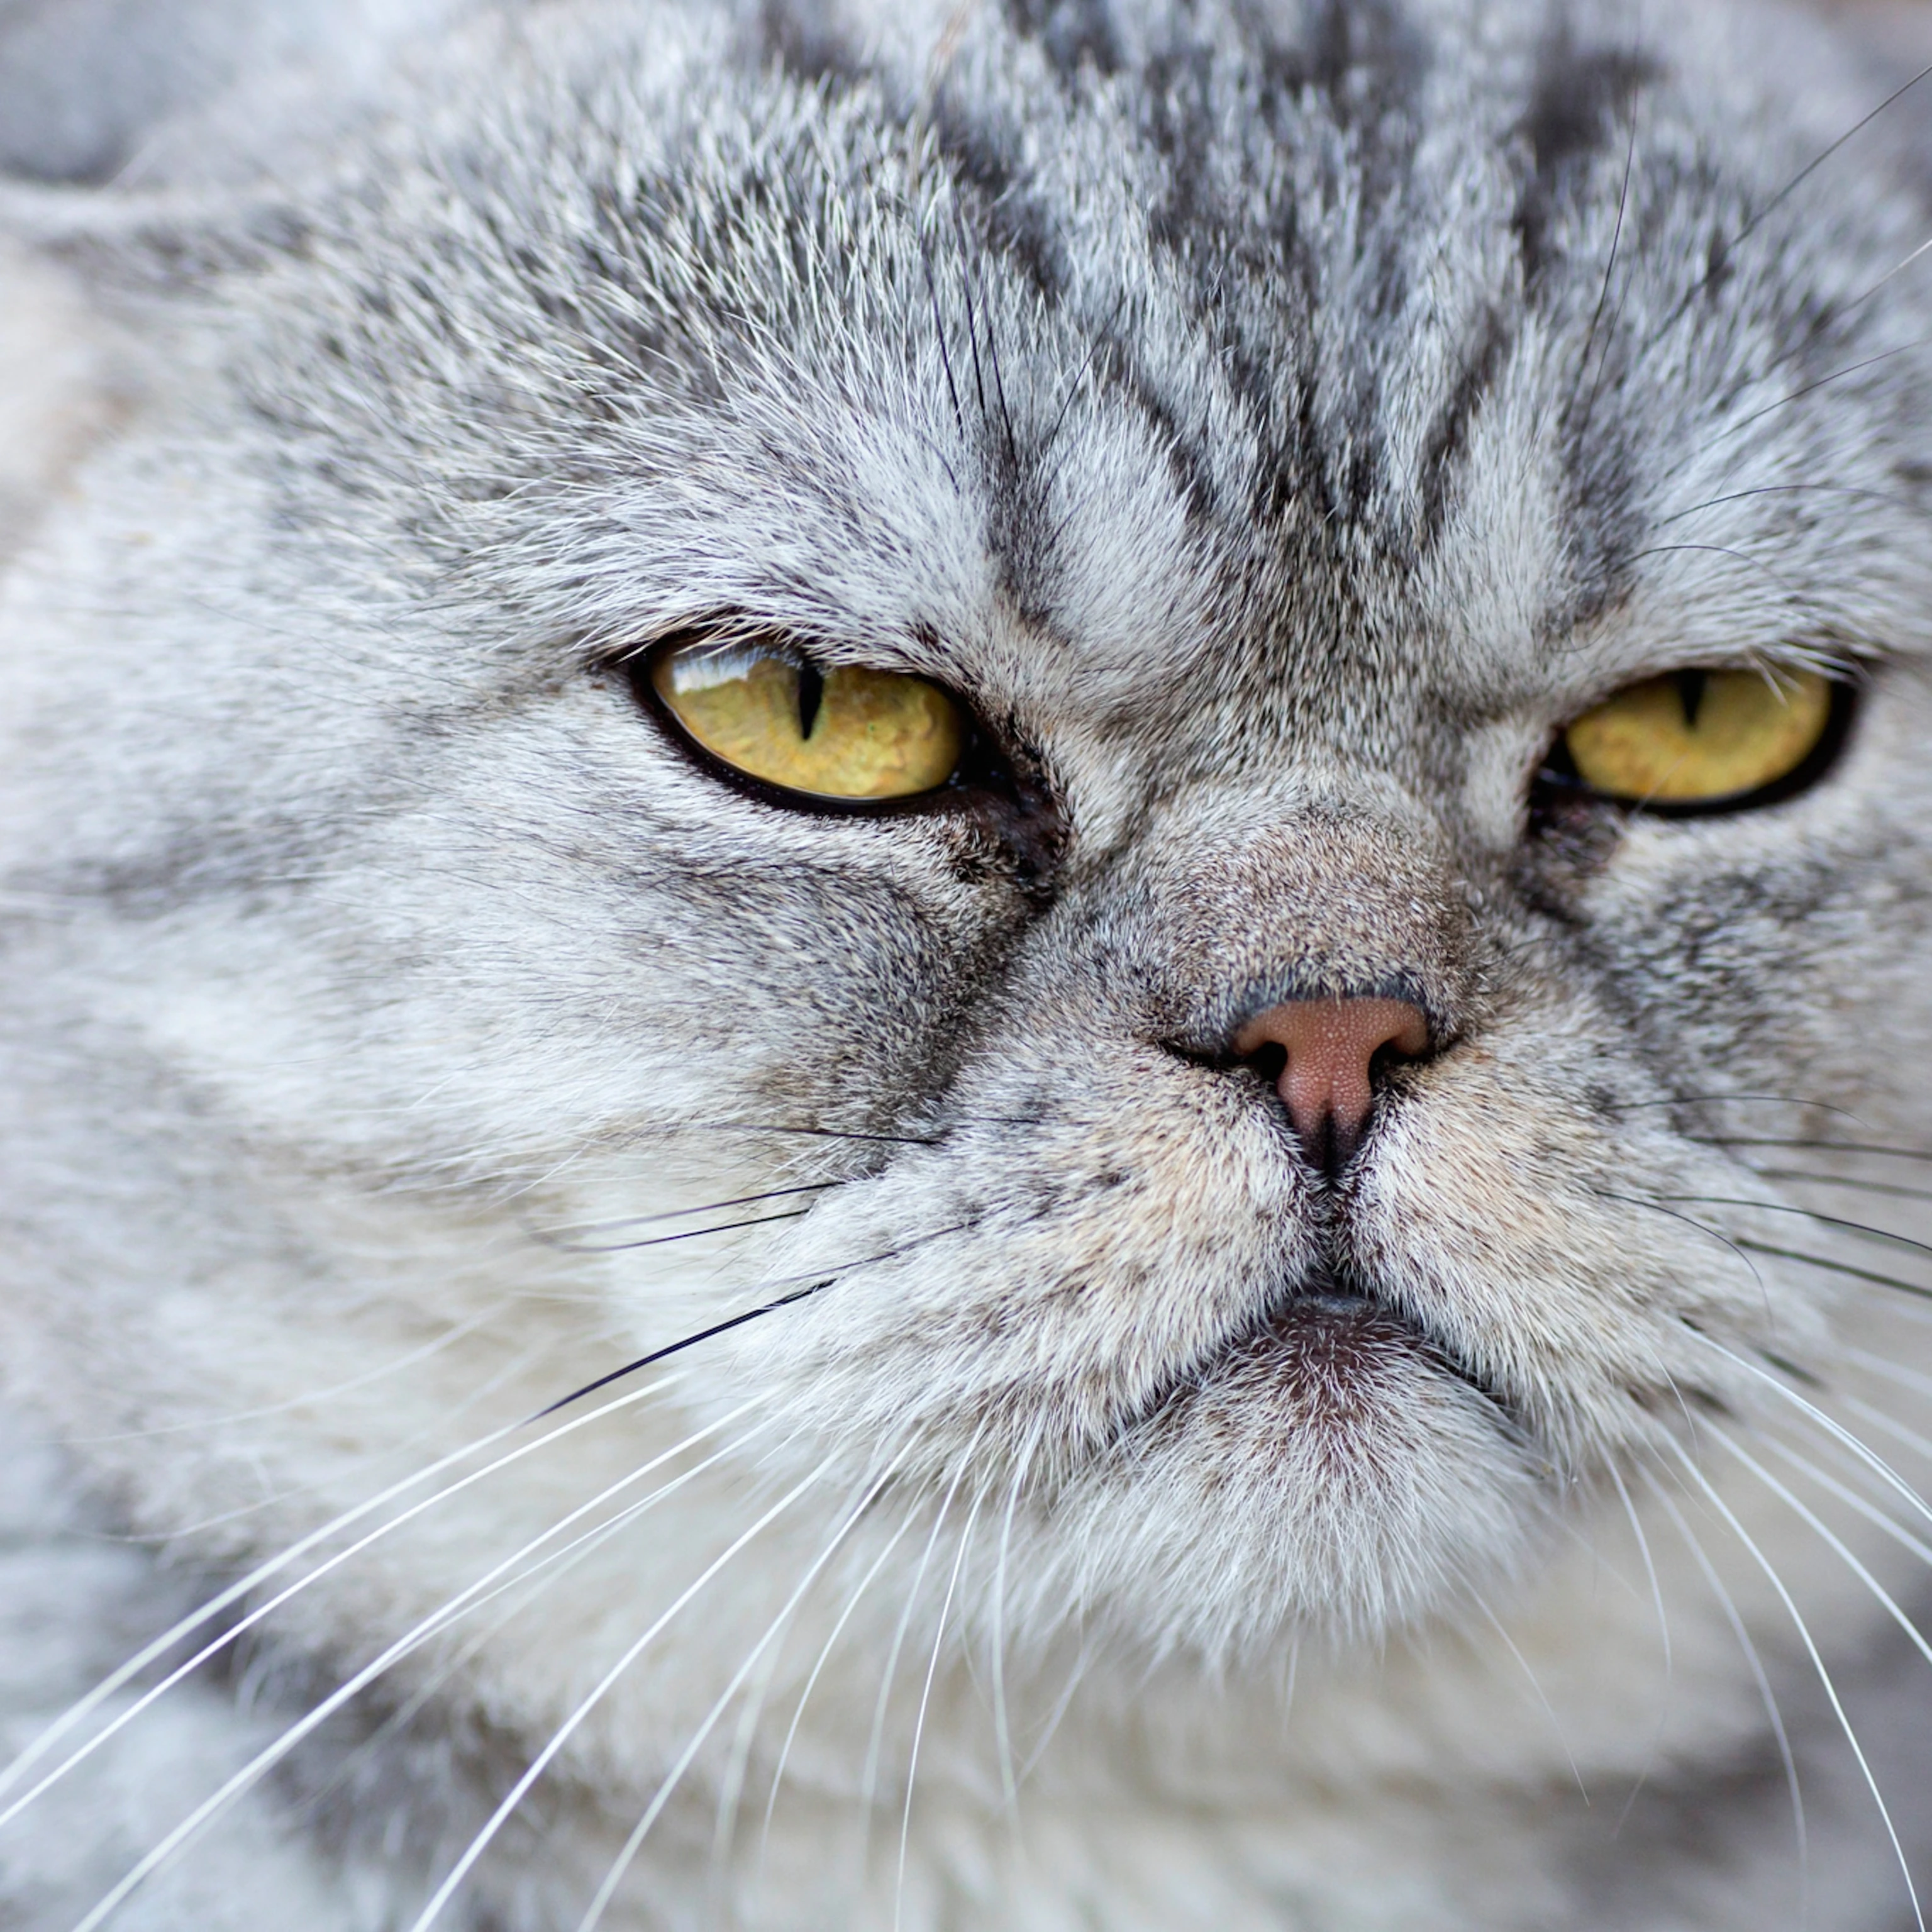
\includegraphics[width=.69\textwidth]{src/images/cat.png}
				\caption{Kat, nogal slechtgezind blijkbaar.}
				\label{fig:kat}
			\end{figure}
			Einde afbeelding 1.
			
		\subsection{Opmerking bij tabellen en figuren}
			Merk op dat de figuur en tabellen niet meteen staan waar je verwacht. Zo staat afbeelding 1 niet tussen de tekst ook al staat hij in de broncode wel tussen de tekst. Dit is omdat deze geplaatst worden waar latex denkt dat ze het best staan. 
			Als je dit perse wil veranderen, kan je dat doen via \texttt{[H]} en de package \texttt{float}.
			Reminder: \ref{subsec:Noot}
		
			\
		
			Begin afbeelding 2.
			\begin{figure}[H]
				\centering
				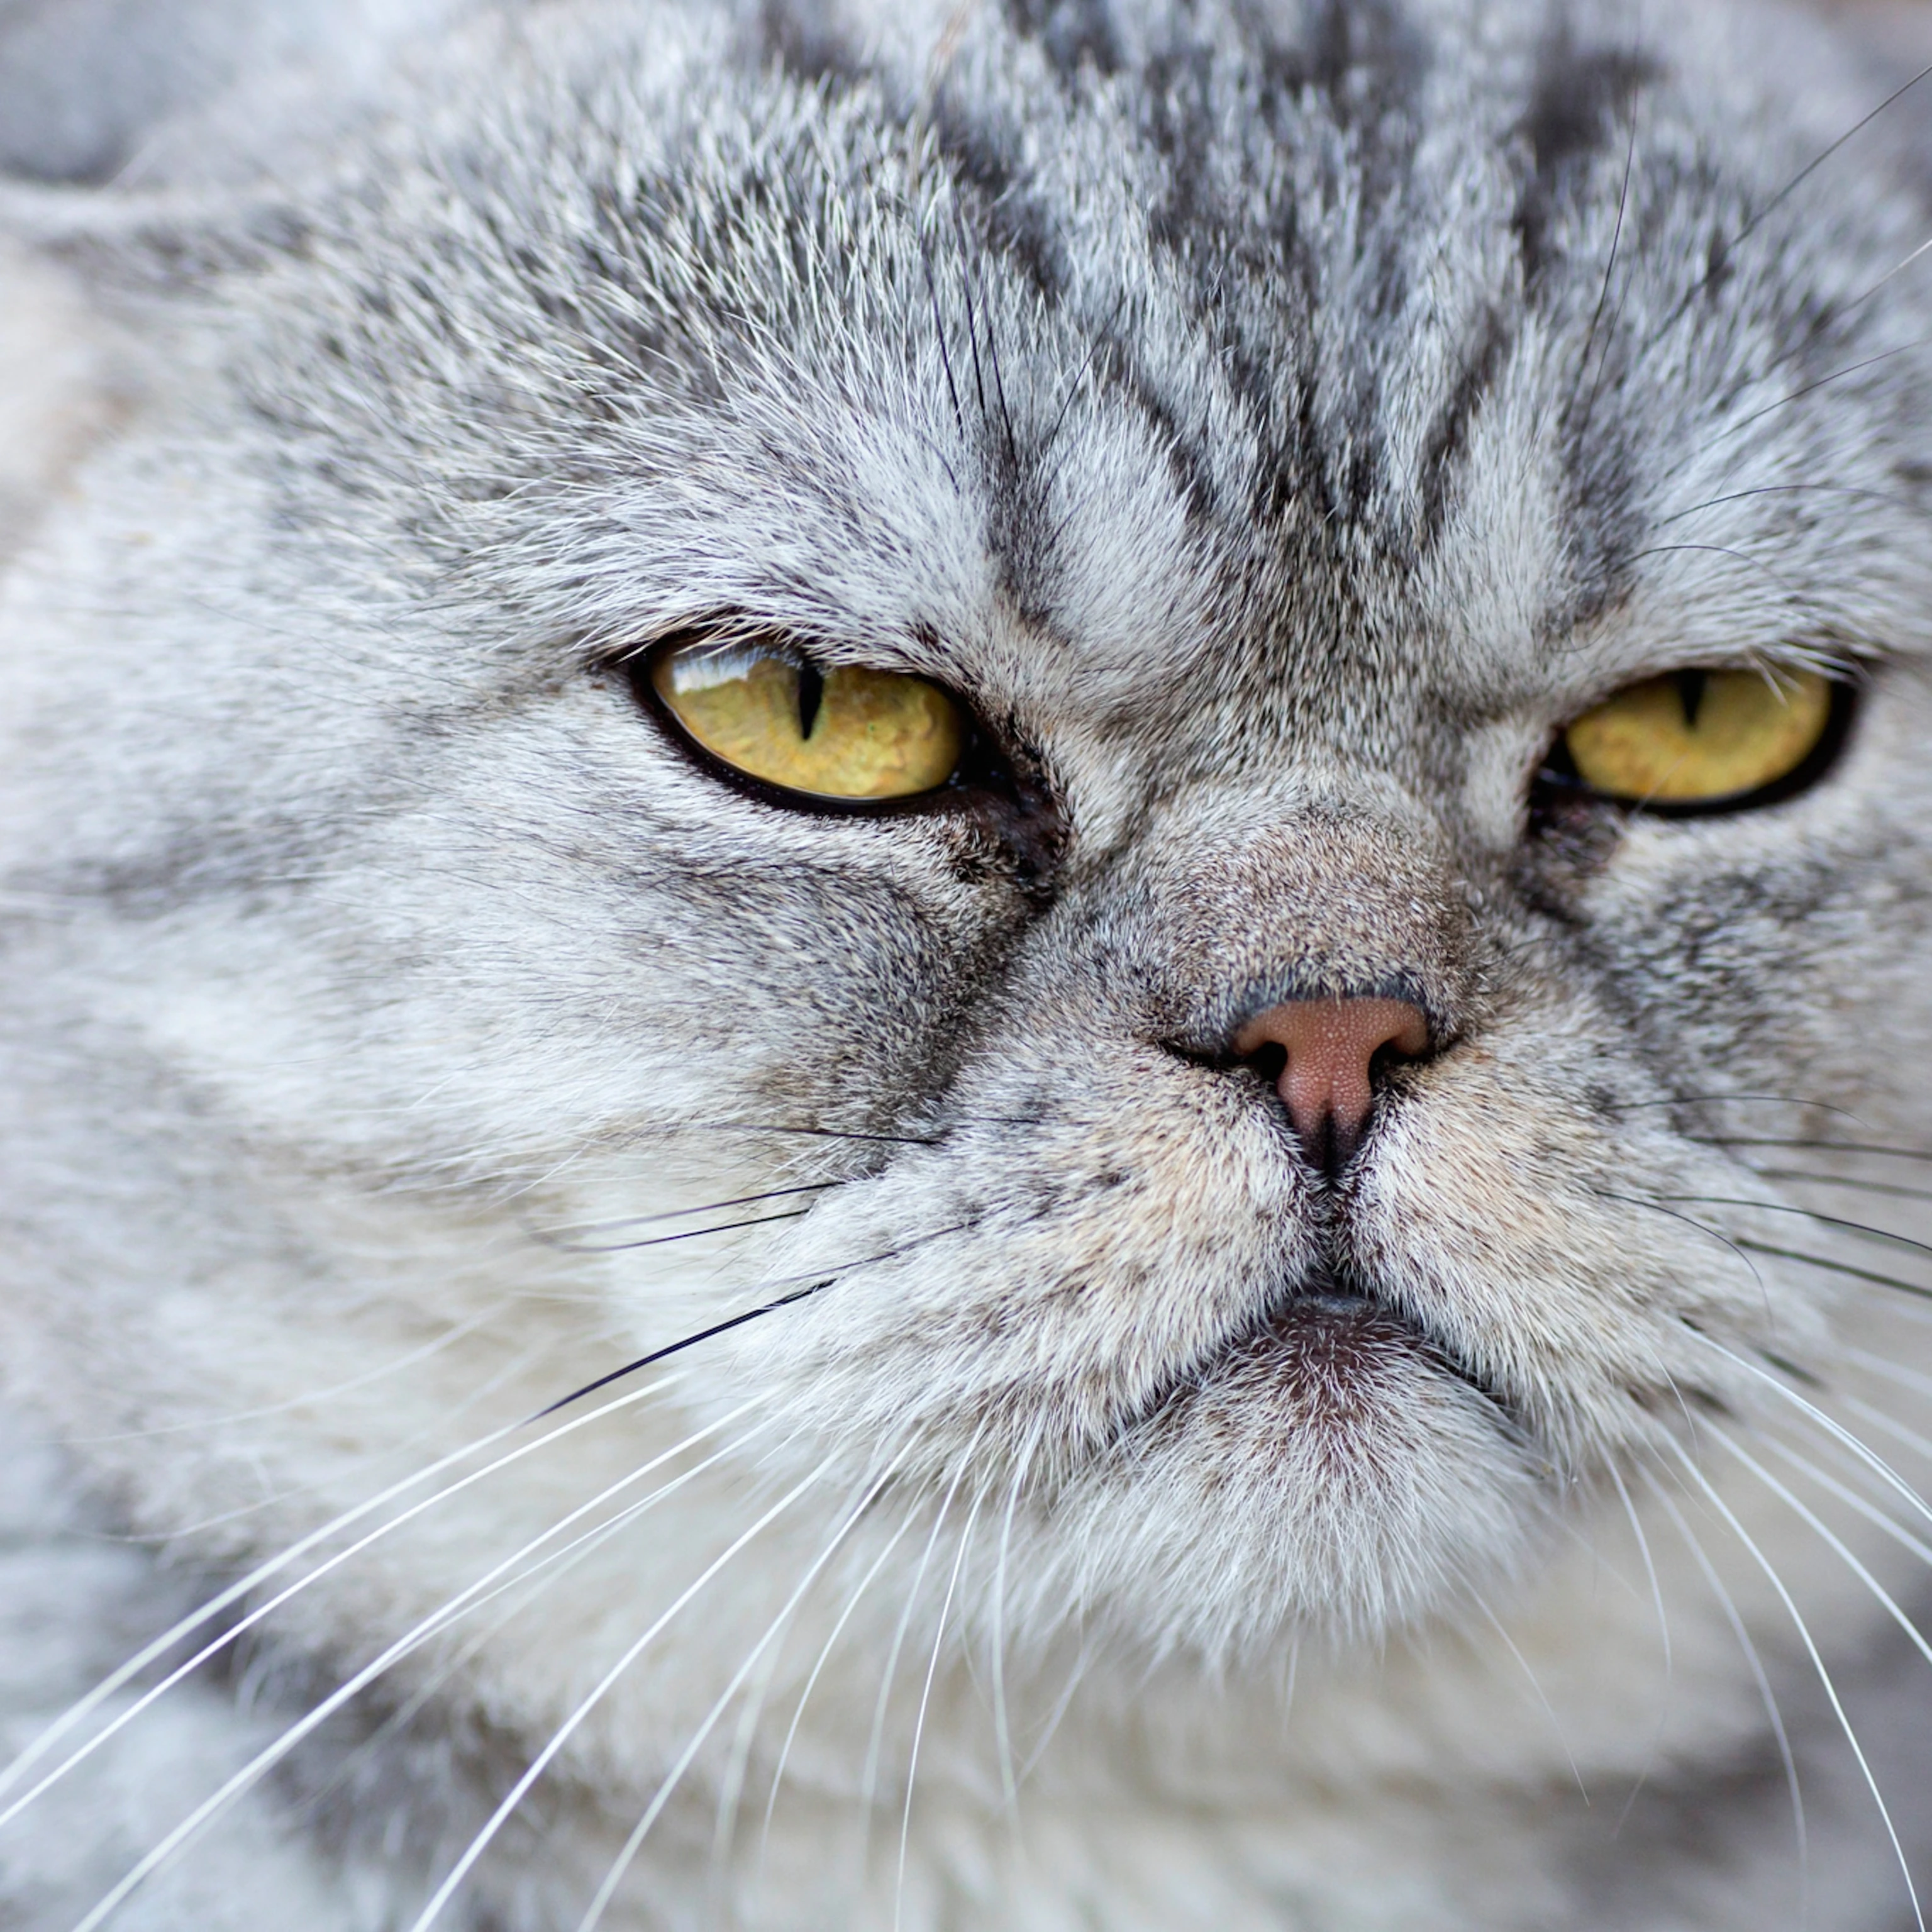
\includegraphics[width=.69\textwidth]{src/images/cat.png}
				\caption{Kat, nogal slechtgezind blijkbaar.}
				\label{fig:kat2}
			\end{figure}
			Einde afbeelding 2.
			
	\section{Verwijzingen en bronvermelding}
		\label{sec:verwijzingenBronvermelding}
		
		\subsection{Verwijzingen}
			Je kunt verwijzen naar eender waar zolang je het \texttt{label} commando gebruikt op de bestemming.
			Je kiest best een goede naam, bijvoorbeeld \texttt{\textit{categorie}:\textit{goede\_naam}}
			Daarna kan je simpelweg gebruik maken van het \texttt{ref} commando om te verwijzen.
			\footnote{Deze refs zijn wederom klikbaar dankzij de package \texttt{hyperref}.}
			
			Deze referenties passen zich ook automatisch aan van stijl afhankelijk van waar het \texttt{label} staat, zo zien verwijzingen naar secties er zo \ref{subsubsec:subsubsec} uit, waar verwijzing naar figuren er dan weer zo \ref{fig:kat} uit zien.
			
		\subsection{Bronvermelding}
			Er zijn meerdere verschillende manieren om bronvermelding te doen. De meest courante leg ik uit.
			
			\subsubsection{In de tekst}
				Voor bronvermelding in een tekst kun je het commando \texttt{cite} gebruiken. Bijvoorbeeld:
			
				Een zeer goede handleiding voor \LaTeX is The not so short introduction \cite{oetiker1995not}. Voor beamer is de user manual \cite{tantau2004user} verplichte kost
			
			\subsubsection{Niet in de tekst}
				Het commando \texttt{nocite} kan gebruikt worden om een bron te doen verschijnen in je bronnenlijst, zonder dat je deze specifiek ergens vermeld in je tekst.
				\nocite{wikipedia:LaTeX}
	
			\subsubsection{Bronnenlijst}
				Een bronnenlijst maak je met het commando \texttt{bibliography}
				
				% Naam van de .bib file met je bronnen
				\bibliography{mainBibliography.bib}
				
		\subsection{Include}
			\subsubsection{Include pdf}
				Met \texttt{includepdf} kun je een andere pdf in het document plaatsen.
				
				\includepdf[pages=-]{src/pdfs/include.pdf}

			\subsection{Include}
				Met \texttt{include} kun je een ander tex bestand invoegen in dit document.
				Dit is handig om bijvoorbeeld met git te werken, aangezien je de file opsplitst zijn er minder merge conflicts.
				
				\
				
				Het commando \texttt{input} doet hetzelfde als include, maar zonder een nieuwe pagina te starten.
				
	\section*{Voorbeelden include}
	
	Tekst voor include.			
	\include{sections/exampleIncludeSection1.tex}
	Tekst na include
	
	Tekst voor input.
	\section*{Voorbeeld include}
    Dit is een Voorbeeld van een section die in een andere file zit.


    \

    Merk op dat input gewoon wordt ingevoegd tussen de bestaande tekst, zonder nieuwe pagina's te maken.

	Tekst na input.
	\section*{Voorbeeld include}
    Dit is een Voorbeeld van een section die in een andere file zit.

    \

    Merk op dat citeringen, vb. \cite{oetiker1995not}, en referenties, vb. \ref{sec:verwijzingenBronvermelding}, \ref{sec:exampleInclude1}, gewoon werken, ookal zitten ze in een ander bestand.

	
	\section{Varia}
		\subsection{git}
			Om het werken met git beter te maken, is het aangeraden om elke zin op een nieuwe regel te starten.
			Dit heeft geen invloed op de effectieve lay-out van het document.
			Het zorgt er wel voor dat er minder merge conflicten zijn.
			Dit is zo omdat het git algoritme werkt op lijn-basis.
			Deze tekst is geschreven op een goeie manier voor git.
			
			\
			
			
			Om het werken met git beter te maken, is het aangeraden om elke zin op een nieuwe regel te starten. Dit heeft geen invloed op de effectieve lay-out van het document. Het zorgt er wel voor dat er minder merge conflicten zijn. Dit is zo omdat het git algoritme werkt op lijn-basis. Deze tekst is geschreven op een slechte manier voor git.
							
\end{document}